%!TEX root = ../main.tex
\documentclass[float=false, crop=false]{standalone}
\usepackage[subpreambles=true]{standalone}
\begin{document}

\section{Timeline and Risks}
% \subsection{Timeline}

\begin{figure}[h!]
    \begin{center}
        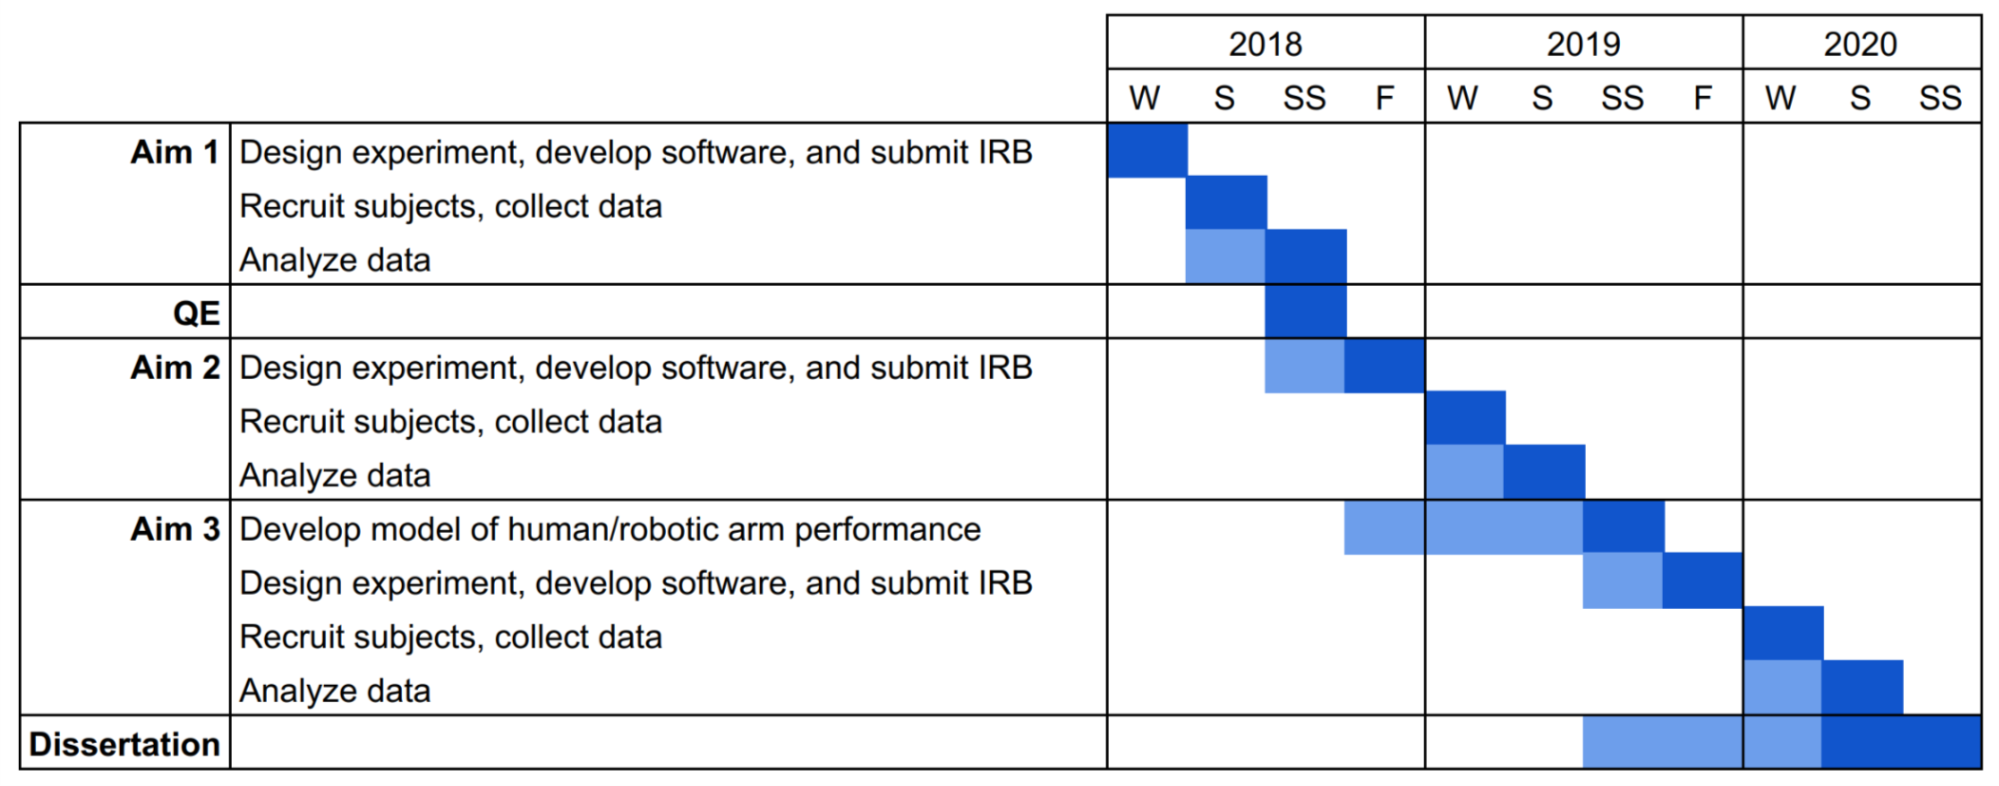
\includegraphics[width=\linewidth]{./../img/image1.png}
        \caption{The Proposed Timeline for this Research}
        \label{timeline}
    \end{center}
\end{figure}

The proposed timeline for the remainder of this research is available in Figure~\ref{timeline}.
This timeline shows the past few months spent accomplishing the first aim and outlines our estimated timeline to complete the following aims, with an estimated graduation date of Summer Quarter 2020.
While not present on the timeline, we also plan to write and submit several additional conference papers and journal articles throughout the completion of this research.

A conference paper, ``Evaluating Augmented Reality in a Three-Axis Manual Tracking Task'', J. Karasinski and S. Robinson has recently been submitted for consideration at AIAA SciTech 2018.
A draft journal article on the SAFER experiment is being prepared for submission in the journal of Human Factors.
We expect to publish an additional conference paper to an AIAA or IEEE conference and journal article for the results of the robotic arm experiment, likely in Human Factors.
If we are successful in creating a model which closely follows human behavior, we would also expect to publish this as a journal article, likely in the Journal of Guidance, Control, and Dynamics.

% \subsection{Risks}
This timeline was created under the assumption that everything will go according to plan, which is almost certainly not the case.
There are a number of places where we may suffer delays or other issues:
\begin{itemize}
\item It is difficult to predict, for instance, how long it will take to recruit subjects and run them through an experiment.
Under the assumption that we will run approximately twenty to thirty subjects in the robotic arm experiment, and that the experiment will last for approximately two to three hours, we have budgeted one quarter to recruit subjects and run them through the experiment.
This could, however, easily stretch to two quarters, depending on subject availability and success rates.
\item NASA Ames has agreed to allow me to use the ROBoT simulator for this proposed experiment and has said that I can bring the simulator to Davis.
There may fall through, of course, at which point I could either run the experiment at Ames or attempt to build my own simulation.
\item While we believe we have sufficient evidence that our feedback techniques will improve performance, it is also possible that we will not see significant effects in the robotic arm task.
If this is the case we will need to further investigate how this task is different from our previous successes.
This would allow us, for instance, to make begin to make recommendations for which types of tasks can benefit from this feedback.
\item It is possible that we may be unable to create a model which incorporates feedback and that accurately mirrors the effects we have seen in our experiments. This may require us to investigate other types of performance models or to create a novel technique.
\end{itemize}

\end{document}